\chapter{Related projects}
\label{ch:relatedProjects}

As discussed in the introduction, the high-level output of this project is Butter, a peer-to-peer framework and networking stack for building decentralised applications. In this section of the report we will look at other similar projects that were a source of inspiration and helped inform this work. For the related work and literature review of a specific problem in designing peer-to-peer distributed systems refer to Section~\ref{ch:buildingButter}.

Many of the early peer-to-peer networks were popularised by file sharing systems such as Gnutella\cite{gnu2022gnutella}, Napster\cite{tucows2004napster, bartsch2017napster} and the BitTorrent protocol\cite{cohen2008bittorrent}. Peer-to-peer architectures provided new means of accessing and sharing information with a greater degree of freedom as the networks were not governed by any single institution. However, this freedom came at a cost were shared information could break copyright law, and it was inherently very difficult to hold any single individual accountable\cite{benkler2016degrees}. No single organisation or entity was responsible for the system's infrastructure as users would contribute their personal resources. This method of networking and information propagation has since been adopted by various other systems such as mobile `ad-hoc' networks and peer-to-peer sensor networks\cite{ramaswamy2005clustering}.

% Note that this list of projects is not exhaustive and there are many other interesting peer-to-peer project such as the Maidsafe network, Dat project and many forms of this technology can be found in mobile `ad-hoc' networks.


\section{Gnutella}
\label{sec:gnutella}

Gnutella is, or rather was, a peer-to-peer file sharing system. It was initially developed by Justin Frankel and Tom Pepper at a subsidiary of AOL and released in March 2000. Within 24h of its release, AOL attempted to take down the network over concerns about the copyright liability of a platform created to freely share files. However, Gnutella was released as open source software under the GNU General Public Licence\cite{gpl} and AOL were unable to take it down before copies were made. Gnutella was quickly adopted and developed by diverse groups, becoming the basis for a range of peer-to-peer networks. Despite AOL's attempts to take it down, the ball was set in motion giving rise to what would become the first large scale peer-to-peer network\cite{benkler2016degrees}. Over the next decade, Gnutella would be the subject of large amounts of research and work to improve its performance and efficiency\cite{lua2005survey}.

\begin{figure}[ht]
    \centering
    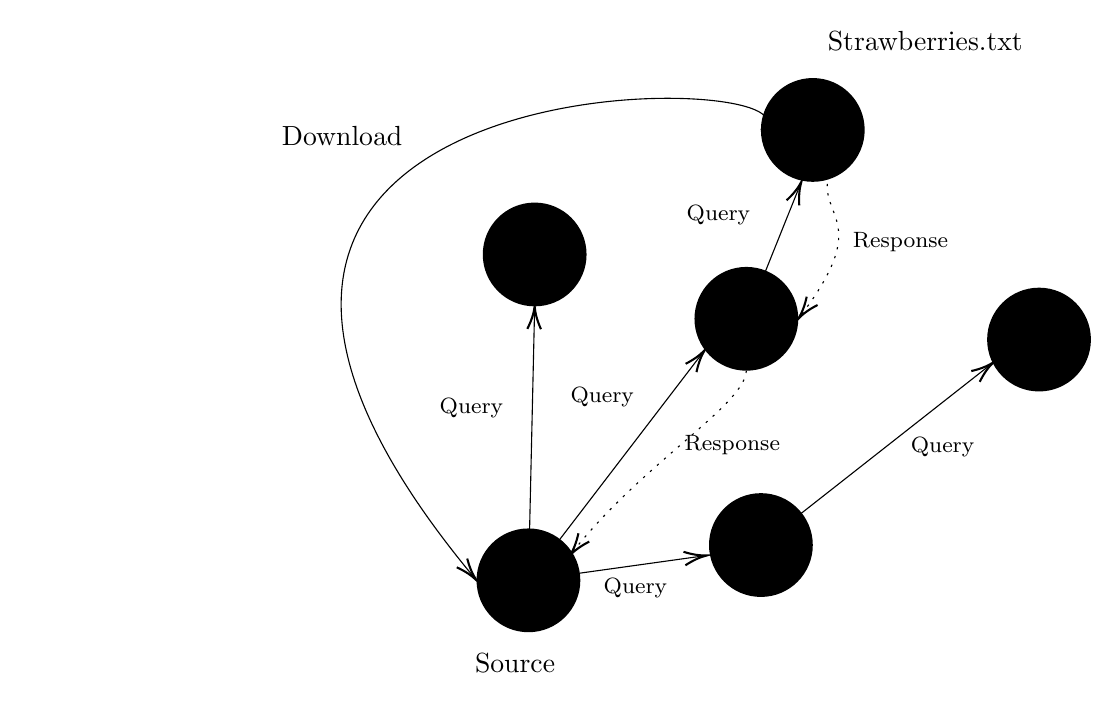
\begin{tikzpicture}[x=0.75pt,y=0.75pt,yscale=-1,xscale=1]
%uncomment if require: \path (0,451); %set diagram left start at 0, and has height of 451

%Shape: Circle [id:dp5701216218873355] 
\draw  [draw opacity=0][fill={rgb, 255:red, 0; green, 0; blue, 0 }  ,fill opacity=1 ] (100,126) .. controls (100,112.19) and (111.19,101) .. (125,101) .. controls (138.81,101) and (150,112.19) .. (150,126) .. controls (150,139.81) and (138.81,151) .. (125,151) .. controls (111.19,151) and (100,139.81) .. (100,126) -- cycle ;
%Shape: Circle [id:dp6701758191642804] 
\draw  [draw opacity=0][fill={rgb, 255:red, 0; green, 0; blue, 0 }  ,fill opacity=1 ] (202,157) .. controls (202,143.19) and (213.19,132) .. (227,132) .. controls (240.81,132) and (252,143.19) .. (252,157) .. controls (252,170.81) and (240.81,182) .. (227,182) .. controls (213.19,182) and (202,170.81) .. (202,157) -- cycle ;
%Shape: Circle [id:dp06164798754338219] 
\draw  [draw opacity=0][fill={rgb, 255:red, 0; green, 0; blue, 0 }  ,fill opacity=1 ] (209,266) .. controls (209,252.19) and (220.19,241) .. (234,241) .. controls (247.81,241) and (259,252.19) .. (259,266) .. controls (259,279.81) and (247.81,291) .. (234,291) .. controls (220.19,291) and (209,279.81) .. (209,266) -- cycle ;
%Shape: Circle [id:dp8491121482645921] 
\draw  [draw opacity=0][fill={rgb, 255:red, 0; green, 0; blue, 0 }  ,fill opacity=1 ] (97,283) .. controls (97,269.19) and (108.19,258) .. (122,258) .. controls (135.81,258) and (147,269.19) .. (147,283) .. controls (147,296.81) and (135.81,308) .. (122,308) .. controls (108.19,308) and (97,296.81) .. (97,283) -- cycle ;
%Shape: Circle [id:dp21625012916250363] 
\draw  [draw opacity=0][fill={rgb, 255:red, 0; green, 0; blue, 0 }  ,fill opacity=1 ] (343,167) .. controls (343,153.19) and (354.19,142) .. (368,142) .. controls (381.81,142) and (393,153.19) .. (393,167) .. controls (393,180.81) and (381.81,192) .. (368,192) .. controls (354.19,192) and (343,180.81) .. (343,167) -- cycle ;
%Shape: Circle [id:dp13339461282709586] 
\draw  [draw opacity=0][fill={rgb, 255:red, 0; green, 0; blue, 0 }  ,fill opacity=1 ] (234,66) .. controls (234,52.19) and (245.19,41) .. (259,41) .. controls (272.81,41) and (284,52.19) .. (284,66) .. controls (284,79.81) and (272.81,91) .. (259,91) .. controls (245.19,91) and (234,79.81) .. (234,66) -- cycle ;
%Straight Lines [id:da3027711082216963] 
\draw    (122,283) -- (124.95,153) ;
\draw [shift={(125,151)}, rotate = 91.3] [color={rgb, 255:red, 0; green, 0; blue, 0 }  ][line width=0.75]    (10.93,-3.29) .. controls (6.95,-1.4) and (3.31,-0.3) .. (0,0) .. controls (3.31,0.3) and (6.95,1.4) .. (10.93,3.29)   ;
%Straight Lines [id:da7950984523527296] 
\draw    (122,283) -- (205.78,173.59) ;
\draw [shift={(207,172)}, rotate = 127.44] [color={rgb, 255:red, 0; green, 0; blue, 0 }  ][line width=0.75]    (10.93,-3.29) .. controls (6.95,-1.4) and (3.31,-0.3) .. (0,0) .. controls (3.31,0.3) and (6.95,1.4) .. (10.93,3.29)   ;
%Straight Lines [id:da09130077482969812] 
\draw    (227,157) -- (252.75,92.86) ;
\draw [shift={(253.5,91)}, rotate = 111.88] [color={rgb, 255:red, 0; green, 0; blue, 0 }  ][line width=0.75]    (10.93,-3.29) .. controls (6.95,-1.4) and (3.31,-0.3) .. (0,0) .. controls (3.31,0.3) and (6.95,1.4) .. (10.93,3.29)   ;
%Straight Lines [id:da12456388559739229] 
\draw    (122,283) -- (206.02,271.28) ;
\draw [shift={(208,271)}, rotate = 172.06] [color={rgb, 255:red, 0; green, 0; blue, 0 }  ][line width=0.75]    (10.93,-3.29) .. controls (6.95,-1.4) and (3.31,-0.3) .. (0,0) .. controls (3.31,0.3) and (6.95,1.4) .. (10.93,3.29)   ;
%Straight Lines [id:da07990008290925488] 
\draw    (234,266) -- (344.43,179.24) ;
\draw [shift={(346,178)}, rotate = 141.84] [color={rgb, 255:red, 0; green, 0; blue, 0 }  ][line width=0.75]    (10.93,-3.29) .. controls (6.95,-1.4) and (3.31,-0.3) .. (0,0) .. controls (3.31,0.3) and (6.95,1.4) .. (10.93,3.29)   ;
%Curve Lines [id:da429610739418806] 
\draw  [dash pattern={on 0.84pt off 2.51pt}]  (266,92) .. controls (265.01,108.83) and (285.58,112.92) .. (253,155.69) ;
\draw [shift={(252,157)}, rotate = 307.69] [color={rgb, 255:red, 0; green, 0; blue, 0 }  ][line width=0.75]    (10.93,-3.29) .. controls (6.95,-1.4) and (3.31,-0.3) .. (0,0) .. controls (3.31,0.3) and (6.95,1.4) .. (10.93,3.29)   ;
%Curve Lines [id:da06143305048271208] 
\draw  [dash pattern={on 0.84pt off 2.51pt}]  (227,182) .. controls (226.01,198.83) and (177,226.44) .. (143.02,269.68) ;
\draw [shift={(142,271)}, rotate = 307.69] [color={rgb, 255:red, 0; green, 0; blue, 0 }  ][line width=0.75]    (10.93,-3.29) .. controls (6.95,-1.4) and (3.31,-0.3) .. (0,0) .. controls (3.31,0.3) and (6.95,1.4) .. (10.93,3.29)   ;
%Curve Lines [id:da928537814793256] 
\draw    (234,66) .. controls (274,36) and (-119,25) .. (97,283) ;
\draw [shift={(97,283)}, rotate = 230.06] [color={rgb, 255:red, 0; green, 0; blue, 0 }  ][line width=0.75]    (10.93,-3.29) .. controls (6.95,-1.4) and (3.31,-0.3) .. (0,0) .. controls (3.31,0.3) and (6.95,1.4) .. (10.93,3.29)   ;

% Text Node
\draw (265,17) node [anchor=north west][inner sep=0.75pt]   [align=left] {Strawberries.txt};
% Text Node
\draw (78,194) node [anchor=north west][inner sep=0.75pt]   [align=left] {{\footnotesize Query}};
% Text Node
\draw (141,189) node [anchor=north west][inner sep=0.75pt]   [align=left] {{\footnotesize Query}};
% Text Node
\draw (197,101) node [anchor=north west][inner sep=0.75pt]   [align=left] {{\footnotesize Query}};
% Text Node
\draw (305,213) node [anchor=north west][inner sep=0.75pt]   [align=left] {{\footnotesize Query}};
% Text Node
\draw (157,281) node [anchor=north west][inner sep=0.75pt]   [align=left] {{\footnotesize Query}};
% Text Node
\draw (277,114) node [anchor=north west][inner sep=0.75pt]   [align=left] {{\footnotesize Response}};
% Text Node
\draw (196,212) node [anchor=north west][inner sep=0.75pt]   [align=left] {{\footnotesize Response}};
% Text Node
\draw (95,317) node [anchor=north west][inner sep=0.75pt]   [align=left] {Source};
% Text Node
\draw (2,63) node [anchor=north west][inner sep=0.75pt]   [align=left] {Download};


\end{tikzpicture}

    \caption{Gnutella network example}
    \label{fig:gnutella}
\end{figure}

At its core, Gnutella is a protocol for search on a flat topology of nodes. Although files are stored in a centralised fashion, i.e.\ a node is responsible for storing a file not the entire network, Gnutella implements a decentralised model for document location and retrieval. Figure~\ref{fig:gnutella} shows the process of retrieving the \verb+Strawberries.txt+ file on a Gnutella network. In this model, every node is a server and a client; they can both query and deliver information. The network topology is flat and each node shares the same similar functionality, so they can be termed as `peers'.

On the Gnutella network there is no centralised directory and the system does not precisely control the network topology or file placement. The placement of data items is not based on any knowledge of the topology, as in a structured peer-to-peer design. To locate a data item, a node queries its neighbours, and gradually floods the network in a Breadth-first search manner. The lookup query is flooded to all neighbours, and if no match is found, the query is then forwarded to their neighbours. The query is typically bounded to a certain radius which is specified with a Time-to-Live (TTL) flag. This design is resilient to high churn rates, i.e., peers entering and leaving the system\cite{lua2005survey}. However, as the network grows, the search mechanisms do not scale effectively and generate unexpected loads on the network\cite{lua2005survey}.

To join the network, a node initially connects to one of several hosts that are known to be highly available, these are listed on the Gnutella website. This is one of the main weaknesses of the project. While the search mechanism is decentralised and is hence robust and fault-tolerant, the way of first joining and interacting with the network requires a form of centralisation. The ability for new nodes to join is entirely dependent on the availability of the known hosts listed on the Gnutella website. If the known hosts or the website itself were to become unavailable, then no new nodes would be able to join. Having nodes unable to join the network affects the overall probability of the network fulfilling its service.

Once connected to the network, peers can send messages to each other (refer to Figure~\ref{fig:gnutella}). These messages are either directly communicated to all peers with which the sender has open TCP connections or back-propagated, i.e., sent on a specific connection on the reverse of the path taken by an initial broadcast message. Each peer keeps a short cache of the recently routed messages in order to prevent re-broadcasting and to implement back-propagation.\cite{lua2005survey}

% Peers can send the following messages:
% \begin{itemize}
%     \item \textbf{Group Membership} - A peer joining the network broadcasts \verb+PING+ message to announce its presence. The message is then forwarded to its neighbours, initiating back-propagated \verb+PONG+ messages, which contains information about peers, such as the IP address, number and size of the data items.
%     \item \textbf{Search} - A \verb+QUERY+ contains a user specified search string that each receiving peer matches against locally stored file names. The \verb+QUERY+ is broadcasted. \verb+QUERY RESPONSE+ messages are back-propagated replies to \verb+QUERY+ messages and include information necessary to download a file.
%     \item \textbf{File Transfer} - File downloads are performed directly between two peers using these types of messages.
% \end{itemize}

To become a member of the network, a node has to open at least one connection with other peers already on the network. Peers periodically send \verb+PING+ messages to their neighbours to discover other participating peers. A peer decides who to connect to based only on local information. The entire application-level network is composed of peers and open TCP connections as links. The resulting network is a dynamic, self-organised network of independent entities.

Later versions of Gnutella introduced super-peers or ultra-peers\cite{rasti2005long}. These are self-appointed peers with better bandwidth connectivity. Requests are preferentially routed via super-peers, if possible, to help improve the routing performance of the network. However, the design is still limited by the fundamental need to flood large parts of the network to retrieve information.

Finally, while Gnutella laid some of the foundations for implementing a decentralised search mechanism, it does not provide means for improving information availability by having information maintained by the network rather than being strictly tied to a node.

% \cite{ripeanu2001peer} - This could be another good source


\section{JXTA}
\label{sec:jxta}

JXTA\cite{gong2001jxta} was initially released by Sun Microsystems in 2001. It is a network programming and computing platform that is designed to solve a number of problems in distributed computing, especially in peer-to-peer networking\cite{gong2001jxta}. The project was discontinued when Sun was acquired by Oracle in 2009. JXTA provided a network programming platform specifically designed to be the foundation for peer-to-peer systems. The resulting platform was independent of specific transport protocols, languages and application logic.

% \begin{itemize}
%     \item \textbf{Interoperability} - Many of the existing peer-to-peer systems at the time were stricly tied to the user-level application logic, e.g., Napster provided music file sharing and Gnutella provides generic file sharing. There was a lack of common underlying peer-to-peer infrastructure and the resulting systems were incompatible. This meant that existing peer-to-peer communities were duplicating efforts in creating software and system primitives commonly used by all peer-to-peer systems. ``Project JXTA aims to bring to the P2P world what HTTP and the browser brought to the Internet"\cite{jxta}
%     \item \textbf{Platform independence} - Many P2P systems offer their features or
% services through a set of APIs that are delivered on
% a particular operating system using a specific networking protocol. This requires the same system to be developed several times to service a wide peer-to-peer community. JXTA technology was designed to be independent of pre-
% ferred programming languages, development envi-
% ronments, or deployment platforms
%     \item \textbf{Ubiquity} - be implementable
% on every device with a digital heartbeat, including
% sensors, consumer electronics, PDAs, appliances,
% network routers, desktop computers, data-center
% servers, and storage systems
% \end{itemize}

\begin{figure}[ht]
    \centering
    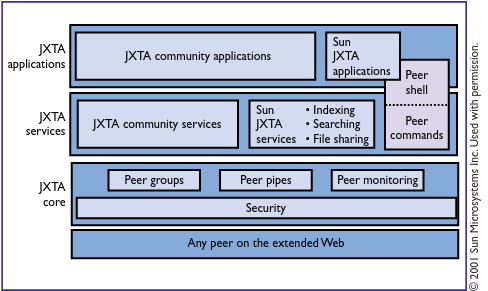
\includegraphics[width=0.7\textwidth]{imgs/Screenshot from 2022-04-16 09-32-03.png}
    \caption{P2P software architecture. JXTA technology provides a layer on top of which services and applications are built. \textit{credit: http://www.jxta.org}}
    \label{fig:jxta_architecture}
\end{figure}

Figure~\ref{fig:jxta_architecture} shows how the JXTA architecture stack breaks down into three layers. At the bottom, the core layer deals with peer establishment, communication management such as routing, and other low-level elements. The six protocols at the JXTA core are listed in Appendix~\ref{jxtaProtocols}. In the middle, a service layer handles higher-level concepts, such as searching and file sharing. The top layer is for application services such as messaging, and storage systems.

% https://ieeexplore.ieee.org/abstract/document/935182


\section{BitTorrent}
\label{sec:bittorrent}

BitTorrent\cite{cohen2008bittorrent} is a centralised peer-to-peer protocol that was originally conceived in 2001 by Bram Cohen. The protocol was designed to deliver a file sharing service similar to that of Gnutella. In BitTorrent, like in Gnutella, the burden of file storage is on the community, however, BitTorrent systems also have central serving nodes that handle location management. This enables much greater performance in information retrieval while maintaining some of the advantages of peer-to-peer architectures, namely, sharing bandwidth and load across the network and mitigating the need for data centres\cite{lua2005survey}.

The protocol is designed to incite contribution by taking a `tit-for-tat' approach where a peer responds with the same action that its other collaborating peer performed previously, e.g., if a node downloads a file hosted by other nodes, it subsequently hosts the file.

\begin{figure}[ht]
    \centering
    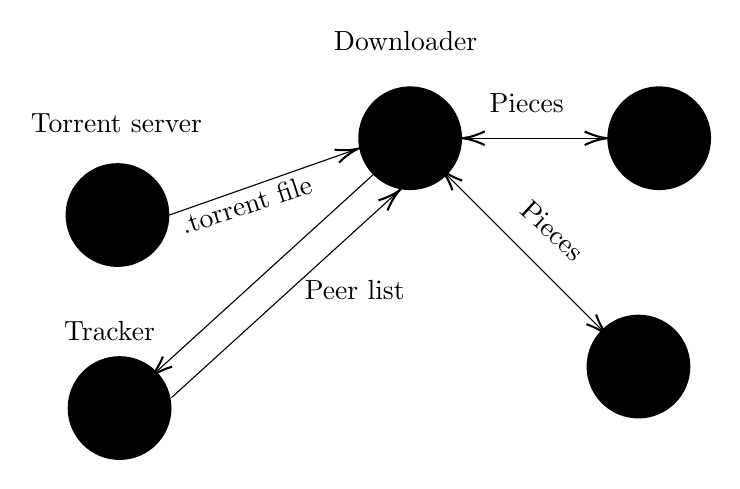
\begin{tikzpicture}[x=0.75pt,y=0.75pt,yscale=-1,xscale=1]
%uncomment if require: \path (0,300); %set diagram left start at 0, and has height of 300

%Shape: Circle [id:dp48020129375115905]
    \draw  [draw opacity=0][fill={rgb, 255:red, 0; green, 0; blue, 0 }  ,fill opacity=1 ] (290,195) .. controls (290,181.19) and (301.19,170) .. (315,170) .. controls (328.81,170) and (340,181.19) .. (340,195) .. controls (340,208.81) and (328.81,220) .. (315,220) .. controls (301.19,220) and (290,208.81) .. (290,195) -- cycle ;
%Shape: Circle [id:dp34478913628095786]
    \draw  [draw opacity=0][fill={rgb, 255:red, 0; green, 0; blue, 0 }  ,fill opacity=1 ] (289,102) .. controls (289,88.19) and (300.19,77) .. (314,77) .. controls (327.81,77) and (339,88.19) .. (339,102) .. controls (339,115.81) and (327.81,127) .. (314,127) .. controls (300.19,127) and (289,115.81) .. (289,102) -- cycle ;
%Shape: Circle [id:dp057127662756395914]
    \draw  [draw opacity=0][fill={rgb, 255:red, 0; green, 0; blue, 0 }  ,fill opacity=1 ] (430,65) .. controls (430,51.19) and (441.19,40) .. (455,40) .. controls (468.81,40) and (480,51.19) .. (480,65) .. controls (480,78.81) and (468.81,90) .. (455,90) .. controls (441.19,90) and (430,78.81) .. (430,65) -- cycle ;
%Shape: Circle [id:dp4152860206319915]
    \draw  [draw opacity=0][fill={rgb, 255:red, 0; green, 0; blue, 0 }  ,fill opacity=1 ] (550,65) .. controls (550,51.19) and (561.19,40) .. (575,40) .. controls (588.81,40) and (600,51.19) .. (600,65) .. controls (600,78.81) and (588.81,90) .. (575,90) .. controls (561.19,90) and (550,78.81) .. (550,65) -- cycle ;
%Shape: Circle [id:dp7865484354927322]
    \draw  [draw opacity=0][fill={rgb, 255:red, 0; green, 0; blue, 0 }  ,fill opacity=1 ] (540,175) .. controls (540,161.19) and (551.19,150) .. (565,150) .. controls (578.81,150) and (590,161.19) .. (590,175) .. controls (590,188.81) and (578.81,200) .. (565,200) .. controls (551.19,200) and (540,188.81) .. (540,175) -- cycle ;
%Straight Lines [id:da837231546510533]
    \draw    (339,102) -- (428.11,70.66) ;
    \draw [shift={(430,70)}, rotate = 160.63] [color={rgb, 255:red, 0; green, 0; blue, 0 }  ][line width=0.75]    (10.93,-3.29) .. controls (6.95,-1.4) and (3.31,-0.3) .. (0,0) .. controls (3.31,0.3) and (6.95,1.4) .. (10.93,3.29)   ;
%Straight Lines [id:da29190602799399223]
    \draw    (440,80) -- (331.48,178.65) ;
    \draw [shift={(330,180)}, rotate = 317.73] [color={rgb, 255:red, 0; green, 0; blue, 0 }  ][line width=0.75]    (10.93,-3.29) .. controls (6.95,-1.4) and (3.31,-0.3) .. (0,0) .. controls (3.31,0.3) and (6.95,1.4) .. (10.93,3.29)   ;
%Straight Lines [id:da7788788491503738]
    \draw    (340,190) -- (448.52,91.35) ;
    \draw [shift={(450,90)}, rotate = 137.73] [color={rgb, 255:red, 0; green, 0; blue, 0 }  ][line width=0.75]    (10.93,-3.29) .. controls (6.95,-1.4) and (3.31,-0.3) .. (0,0) .. controls (3.31,0.3) and (6.95,1.4) .. (10.93,3.29)   ;
%Straight Lines [id:da42573370946311306]
    \draw    (548,65) -- (482,65) ;
    \draw [shift={(480,65)}, rotate = 360] [color={rgb, 255:red, 0; green, 0; blue, 0 }  ][line width=0.75]    (10.93,-3.29) .. controls (6.95,-1.4) and (3.31,-0.3) .. (0,0) .. controls (3.31,0.3) and (6.95,1.4) .. (10.93,3.29)   ;
    \draw [shift={(550,65)}, rotate = 180] [color={rgb, 255:red, 0; green, 0; blue, 0 }  ][line width=0.75]    (10.93,-3.29) .. controls (6.95,-1.4) and (3.31,-0.3) .. (0,0) .. controls (3.31,0.3) and (6.95,1.4) .. (10.93,3.29)   ;
%Straight Lines [id:da47394536708390655]
    \draw    (548.59,158.59) -- (471.41,81.41) ;
    \draw [shift={(470,80)}, rotate = 45] [color={rgb, 255:red, 0; green, 0; blue, 0 }  ][line width=0.75]    (10.93,-3.29) .. controls (6.95,-1.4) and (3.31,-0.3) .. (0,0) .. controls (3.31,0.3) and (6.95,1.4) .. (10.93,3.29)   ;
    \draw [shift={(550,160)}, rotate = 225] [color={rgb, 255:red, 0; green, 0; blue, 0 }  ][line width=0.75]    (10.93,-3.29) .. controls (6.95,-1.4) and (3.31,-0.3) .. (0,0) .. controls (3.31,0.3) and (6.95,1.4) .. (10.93,3.29)   ;

% Text Node
    \draw (271,52) node [anchor=north west][inner sep=0.75pt]   [align=left] {Torrent server};
% Text Node
    \draw (287,152) node [anchor=north west][inner sep=0.75pt]   [align=left] {Tracker };
% Text Node
    \draw (417,12) node [anchor=north west][inner sep=0.75pt]   [align=left] {Downloader};
% Text Node
    \draw (341.71,101.92) node [anchor=north west][inner sep=0.75pt]  [rotate=-341.81] [align=left] {.torrent file};
% Text Node
    \draw (403,132) node [anchor=north west][inner sep=0.75pt]   [align=left] {Peer list};
% Text Node
    \draw (492,42) node [anchor=north west][inner sep=0.75pt]   [align=left] {Pieces};
% Text Node
    \draw (513.44,92.15) node [anchor=north west][inner sep=0.75pt]  [rotate=-42.84] [align=left] {Pieces};

\end{tikzpicture}


    \caption{BitTorrent architecture}
    \label{fig:bittorentArchitecture}
\end{figure}

The architecture (depicted in Figure~\ref{fig:bittorentArchitecture}) consists of a central location, called a tracker and many peers. When attempting to download a file from the network a peer initially connects to a known tracker to download a \verb+.torrent+ file. This file contains metadata about the requested file such as its length, name, hashing information and URL of a tracker.

Trackers keep track of all the peers hosting a file using a protocol layered on top of HTTP. A downloader sends information about the file it is downloading to the tracker. The tracker responds with a list of contact information about the peers that are downloading the same file. Downloaders then use this information to connect to each other. A downloader that has the complete file, known as a seed, must send out at least one complete copy of the original file. Each downloader announces to all of its peers which piece of information it has. When a peer finishes downloading a piece, it checks that the hash matches with that of the \verb+.torrent+ file, and announces that it has that piece to all of its peers. This verifies data integrity.

% \section{Beaker browser and Hypercore protocol}

% The Beaker browser is an experimental peer-to-peer web browser which runs a peer process in the background while using a Chromium based browser\cite{beaker}. This allows users to contribute to the network as they are browsing the internet which presents an interesting model of internet consumption and infrastructure. In addition, the browser allows users to publish websites and upload files directly from the browser so that they are available on the peer-to-peer network. The browser provides a high-level GUI enabling ease of use for new users to insight a greater community of users and hence peers.

% Beaker is built on top of the Hypercore protocol, a ``peer-to-peer data network built on Hypercore logs"\cite{hypercore} known as `hypercores'. Hypercore is the evolution of the Dat protocol\cite{ogden2017dat}. Hypercores are signed, append-only logs that can be thought of as a `lightweight' blockchain without the consensus algorithm. Append-only logs can be thought of as arrays in which the operations can only be \verb+get(index)+, \verb+push(data)+ and \verb+retrieve+ but where you can never overwrite pre-existing entries. Using append-only logs, Hypercore can easily generate compressed bitfields describing which portions of a log a peer hosts. This helps make the replication protocol light and efficient\cite{hypercore}.

% Hypercore allows efficient and quick distribution of the logs as each peer can choose to download only the section of the log they are interested in, without having to download everything from the beginning. However, while Hypercore could be a powerful approach to designing peer-to-peer systems it has seen fairly little use in its seven years of development.

% Briefly discuss the trees that they use with cryptography...


\section{libp2p}
\label{sec:libp2p}

\verb+libp2p+, unlike Gnutella or BitTorrent, does not deliver a specific user service but rather provides developers with a platform to build decentralised applications, much like JXTA. As of time of writing, it is used as the underlying peer-to-peer networking stack behind the IPFS project, Filecoin (a cryptocurrency based on sharing files) and the Ethereum cryptocurrency. \verb+libp2p+ is not a single library but rather a continuously maintained specification for the implementation of the peer-to-peer protocols. The project's ambition is to inform and make developing peer-to-peer applications significantly easier in an effort to increase their ubiquity\cite{dias2018IntroLibp2p}.

\begin{figure}[ht]
    \centering
    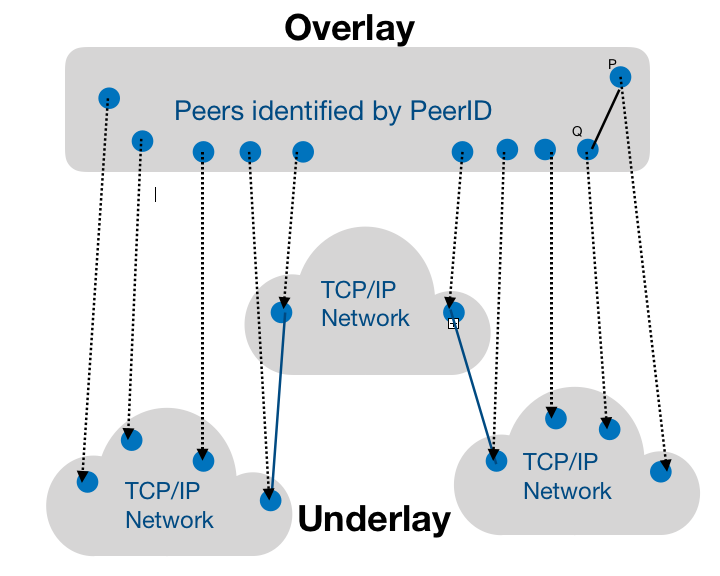
\includegraphics[width=0.5\textwidth]{imgs/0oGSfw7.png}
    \caption{libp2p Peer IDs that are unique across subnetworks}
    \label{fig:libp2pPeerIds}
\end{figure}

The project introduces some interesting innovations such as Peer IDs, which can uniquely identify peers across subnetworks producing an overlay that bridges networks (see Figure~\ref{fig:libp2pPeerIds}). One of the major innovation of \verb+libp2p+ is the introduction of `multiaddresses' which specify a peer and communication protocol in a standard string format. This allows the address to not only imply a recipient but also the protocol for addressing it. Peers can hence form connection between each other with many protocols for different scenarios. The connection between peers in \verb+libp2p+ is called a stream. More than one stream can be active between the same pair of peers, and each stream is logically independent of one another. When a new stream is opened, the two peers can negotiate which protocols should be used, and when a peer proposes a protocol to use, the other can accept it or send a message saying that it does not support it. When a consensus is reached, the peers will start using the agreed upon protocol.\cite{guidi2021libp2p}

To discover new peers in the network, \verb+libp2p+ uses multicast broadcasting for local peers and boostrap endpoints that enable the peer to be discovered by the wider network. When a peer is online, it can observe the network to learn which are the most reliable peers, i.e., highly available peers. By storing their IDs in a bootstrap list it can then readily join the network again without a prompted boostrap endpoint. Peers can share information about highly available nodes between themselves. This approach introduces some central points of failure in the discovery mechanisms, however, \verb+libp2p+ offers a fault-tolerant solution by providing several discovery mechanisms and relying on rendezvous as a fallback.

For NAT traversal \verb+libp2p+ offers several protocols. If the router supports UPnP (Universal Plug and Play) or nat-pmp (NAT Port Mapping Protocol), \verb+libp2p+ automatically tries to configure the router to enable inbound traffic. Another techniques used by \verb+libp2p+ is to listen to incoming connection on the same public port of the router as the port associated by the router to the peer's outbound connections. While these are far from perfect solutions, they are some of the best options currently available. NAT traversal could be avoided with wider adoption of the IPv6 protocol by Internet service providers (ISPs). IPv6 allows for the unique identification of all internet connected devices, but for the moment, most ISPs do not support the new protocol.

\verb+libp2p+ offers three protocols for content routing: Multicast DNS (mDNS), Kademlia DHT (KAD), and Publish-Subscribe. mDNS consists of broadcasting a query and asking local peers to identify themselves, while KAD leverages a Distributed Hash Table to find a peer with specific content. The Publish-Subscribe protocol has two implementations: FloodSub (based on network flooding) and GossipSub. In GossipSub peers are organised in a 2-layer logical network: a sparse layer, called full-message, where the published messages are exchanged using gossiping algorithms, and a dense layer, called metadata-only, used to maintain the other layer.\cite{guidi2021libp2p}

\begin{figure}[ht]
    \centering
    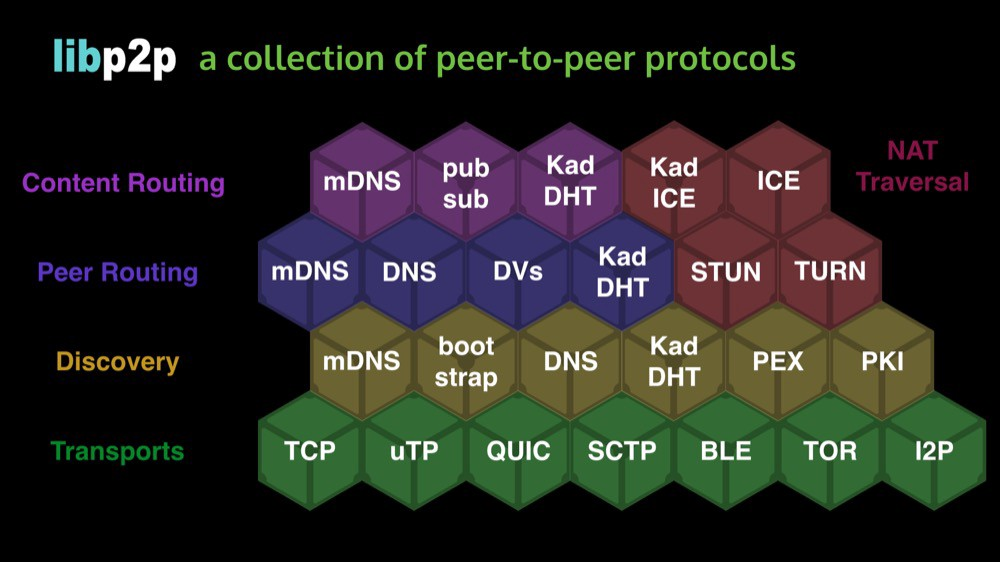
\includegraphics[width=0.7\textwidth]{imgs/libp2p.jpeg}
    \caption{libp2p modules}
    \label{fig:libp2pModules}
\end{figure}

One of the core characteristics of the \verb+libp2p+ project is that it is fundamentally modular this is expressed in their logo and is conveyed throughout their documentation. Each module can be imported separately and independently of any other module and addresses a specific problem in peer-to-peer distributed computing. The \verb+libp2p+ module architecture can be seen in Figure~\ref{fig:libp2pModules}.
